% ACCESSNet architecture diagram
% Compile with: pdflatex accessnet.tex
\documentclass[border=10pt]{standalone}

% --- Helvetica for both text and math ---
\usepackage[scaled]{helvet}
\renewcommand{\familydefault}{\sfdefault}
\usepackage{sfmath}
\usepackage[T1]{fontenc}

\usepackage{tikz}
\usepackage{amsmath,amssymb}
\usetikzlibrary{positioning,arrows.meta,fit,backgrounds,calc}

\definecolor{seqcol}{HTML}{C8E6C9}   % green  - input / output
\definecolor{stemcol}{HTML}{90CAF9}  % blue   - stem conv
\definecolor{convcol}{HTML}{BBDEFB}  % blue   - conv tower
\definecolor{sigcol}{HTML}{FFE0B2}   % orange - signal branches
\definecolor{fusecol}{HTML}{B2DFDB}  % teal   - fusion
\definecolor{headcol}{HTML}{FFCDD2}  % red    - classifier head
\definecolor{outcol}{HTML}{F8BBD0}   % pink   - output

\begin{document}
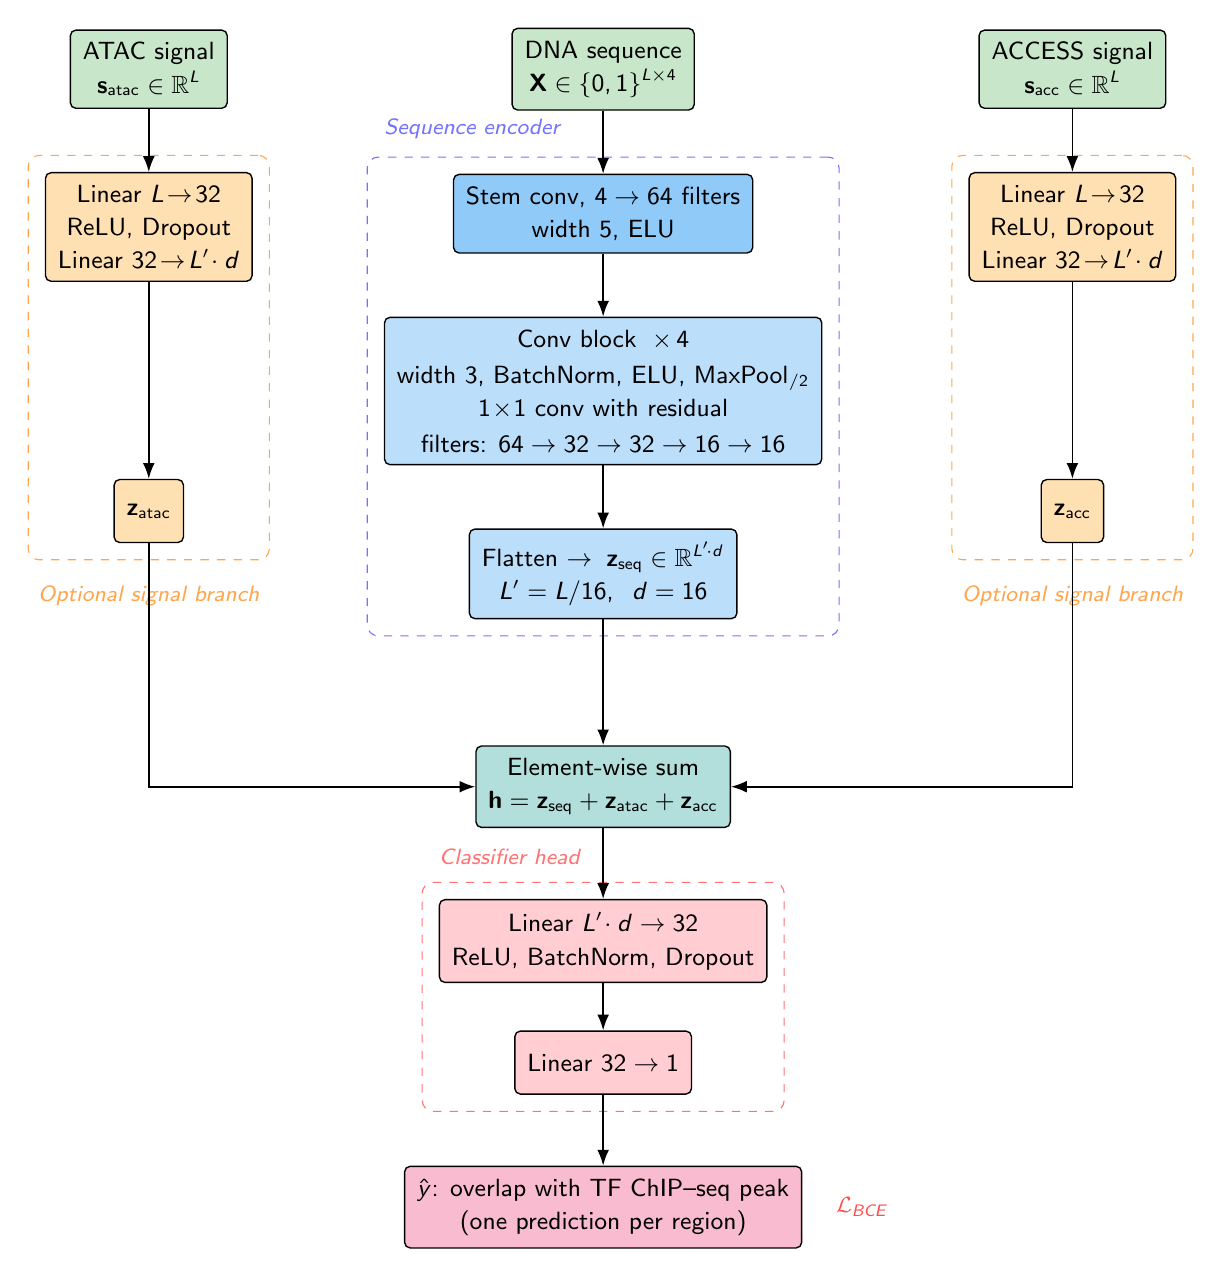
\begin{tikzpicture}[
  font=\small,
  node distance=6mm,
  box/.style={draw, rounded corners=2pt, align=center,
              minimum height=8mm, inner sep=4.5pt, line width=0.5pt},
  arr/.style={-{Latex[length=2mm]}, line width=0.6pt},
  grouplabel/.style={font=\itshape\footnotesize, text=gray},
]

% ---------------------------------------------------------------- inputs
\node[box, fill=seqcol] (dna)
  {DNA sequence\\[1pt] $\mathbf{X}\in\{0,1\}^{L\times 4}$};

\node[box, fill=seqcol, left=36mm of dna] (atacin)
  {ATAC signal\\[1pt] $\mathbf{s}_{\text{atac}}\in\mathbb{R}^{L}$};

\node[box, fill=seqcol, right=36mm of dna] (accin)
  {ACCESS signal\\[1pt] $\mathbf{s}_{\text{acc}}\in\mathbb{R}^{L}$};

% ------------------------------------------------- sequence encoder
\node[box, fill=stemcol, below=8mm of dna] (stem)
  {Stem conv, $4\rightarrow 64$ filters\\[1pt] width 5, ELU};

\node[box, fill=convcol, below=8mm of stem, minimum height=13mm] (tower)
  {Conv block \;$\times\,4$\\[2pt]
   width 3, BatchNorm, ELU, MaxPool$_{/2}$\\[1pt]
   $1\!\times\!1$ conv with residual\\[2pt]
   filters: $64\rightarrow32\rightarrow32\rightarrow16\rightarrow16$};

\node[box, fill=convcol, below=8mm of tower] (zseq)
  {Flatten $\rightarrow\; \mathbf{z}_{\text{seq}}\in\mathbb{R}^{L'\!\cdot d}$\\[1pt]
   $L'=L/16,\;\; d=16$};

\begin{scope}[on background layer]
  \node[draw=blue!55, dashed, rounded corners=4pt, inner sep=6pt,
        fit=(stem)(tower)(zseq)] (seqbox) {};
\end{scope}
\node[grouplabel, anchor=south west, blue!55]
  at ([xshift=1mm,yshift=1mm]seqbox.north west) {Sequence encoder};

% --------------------------------------------------- signal branches
\node[box, fill=sigcol, below=8mm of atacin] (atacmlp)
  {Linear $L\!\rightarrow\!32$\\[1pt] ReLU, Dropout\\[1pt]
   Linear $32\!\rightarrow\!L'\!\cdot d$};
\node[box, fill=sigcol, below=8mm of accin] (accmlp)
  {Linear $L\!\rightarrow\!32$\\[1pt] ReLU, Dropout\\[1pt]
   Linear $32\!\rightarrow\!L'\!\cdot d$};

\node[box, fill=sigcol, below=25mm of atacmlp] (zatac) {$\mathbf{z}_{\text{atac}}$};
\node[box, fill=sigcol, below=25mm of accmlp]  (zacc)  {$\mathbf{z}_{\text{acc}}$};

\begin{scope}[on background layer]
  \node[draw=orange!70, dashed, rounded corners=4pt, inner sep=6pt,
        fit=(atacmlp)(zatac)] (atacbox) {};
  \node[draw=orange!70, dashed, rounded corners=4pt, inner sep=6pt,
        fit=(accmlp)(zacc)] (accbox) {};
\end{scope}
\node[grouplabel, anchor=north, orange!70]
  at ([yshift=-2mm]atacbox.south) {Optional signal branch};
\node[grouplabel, anchor=north, orange!70]
  at ([yshift=-2mm]accbox.south) {Optional signal branch};

% ------------------------------------------------------------- fusion
\node[box, fill=fusecol, below=16mm of zseq] (fuse)
  {Element-wise sum\\[1pt]
   $\mathbf{h}=\mathbf{z}_{\text{seq}}+\mathbf{z}_{\text{atac}}+\mathbf{z}_{\text{acc}}$};

% ------------------------------------------------------------- head
\node[box, fill=headcol, below=9mm of fuse] (fc1)
  {Linear $L'\!\cdot d \rightarrow 32$\\[1pt] ReLU, BatchNorm, Dropout};
\node[box, fill=headcol, below=of fc1] (fc2)
  {Linear $32\rightarrow 1$};

\begin{scope}[on background layer]
  \node[draw=red!55, dashed, rounded corners=4pt, inner sep=6pt,
        fit=(fc1)(fc2)] (headbox) {};
\end{scope}
\node[grouplabel, anchor=south west, red!55]
  at ([xshift=1mm,yshift=1mm]headbox.north west) {Classifier head};

\node[box, fill=outcol, below=9mm of fc2] (out)
  {$\hat{y}$: overlap with TF ChIP--seq peak\\[1pt]
   (one prediction per region)};

\node[grouplabel, right=3mm of out, text=red!70] {$\mathcal{L}_{\text{BCE}}$};

% ------------------------------------------------------------- arrows
\draw[arr] (dna)   -- (stem);
\draw[arr] (stem)  -- (tower);
\draw[arr] (tower) -- (zseq);
\draw[arr] (zseq)  -- (fuse);

\draw[arr] (atacin)  -- (atacmlp);
\draw[arr] (accin)   -- (accmlp);
\draw[arr] (atacmlp) -- (zatac);
\draw[arr] (accmlp)  -- (zacc);
\draw[arr] (zatac) |- (fuse.west);
\draw[arr] (zacc)  |- (fuse.east);

\draw[arr] (fuse) -- (fc1);
\draw[arr] (fc1)  -- (fc2);
\draw[arr] (fc2)  -- (out);

\end{tikzpicture}
\end{document}
